\documentclass[../main.tex]{subfiles}

\begin{document}
\section{CHIPs Architecture}
The CHIPs architecture is an amalgamation of chiplets. Each Chiplet is fabricated separately and connected through an interposer. This structure is known as two and a half Dimensions (2.5D). The CHIPs system contains the following chiplets: two Rocket chips, long short term memory (LSTM) chip, sparse convolutional neural networks (SCNN) chip. Each chaplet has two AXI buses and one Jtag bus. Each AXI bus is broken up into sets of AIB channels. An AIB channel is the physical connection between chiplet and interposer. The Jtag bus uses TSV to connect to interposer.  


%The CHIPs Architecture is a amalgamation of chiplets. This Architecture supports the ability to connect chiplets post die fabrication. Each Chiplet is connected to two AXI buses. One bus is for on and off-chip memory Bus, MBus, and the second bus is the control Bus, XBus. The MBus is the primary bus for memory data transfers. The XBus is used by the Rocket chip to control the neural network chiplet. Figure ?? is overview of the CHIPs Architecture.

%The Chips architecture was designed with the intent of being able to mix and match chips. In order to mix and match chips, the sub-designs (ie. chips) need to be designed in a way that they can be connected through an interposer. This assembly structure is called 2.5D (Physical layer). Figure ?? shows relationship of the die to interposer connections. The SOC is designed to run over-top of AIB. The SOC contains three bus, two are configured as AXI and the other one is configured as CIPI. The SOC connects the ciplets together. There are two types of ciplets: controllers and accelerators.
\subsection{Rocket Chip}

\subsection{Tow and half Dimension Structure}
For most of the connects in the 2.5D structure, an AIB driver makes a face to face connection with the interposer. Each AIB driver makes it possible to transfer data at high speeds. AIB drivers connect in pairs through the interposer. One driver needs to be set to send, and the other needs to be set to receive. Figure ?? shows an overview of an AIB driver. 

An AIB channel consists of 48 AIB drivers.  The lower 40 driver transport data and the upper 8 drivers transport the clock. The clock drivers transmit in different pairs. These four cloks make up the clock forwarding between chiplets. Clock forwarding allows the chiplets to be independent of each chiplet's clock phase. Figure ?? shows the layout of an AIB channel.

\subsection{CHIPS SOC}
The CHIPs SOC uses two protocols: AXI and CIPI. The AXI protocol allows for point to point memory transactions. There are two buses that uses AXI and one bus that uses CIPI. The AXI bus is used for the on-chip and chip to chip commutation. The CIPI bus is used for off-chip commutation. The CIPI bus grows the size of the addressable memory space that that the system can access. With a large address space, larger work loads can be ran. The AXI bus are named XBus and MBus. The MBus connect the global shared memory space for all the chips. The XBus connects all the chips together. Its purpose is used to configure and control the accelerators. Figure ?? show the layout of the buses.

\subsection{Chiplets}
The controllers chiplets use the Rocket Chip IP\cite{Asanović:EECS-2016-17}. In this layout, there are two different layouts for the Rocket Chip, one was wrapped with AIB and the other was not. The two accelerators chiplets are LSTM and SCNN. Figure ?? shows the layout of the tape-out. Each major Design is hi highlighted. 
\subsubsection{Rocket Core}
%\begin{figure}
%    \centering
%    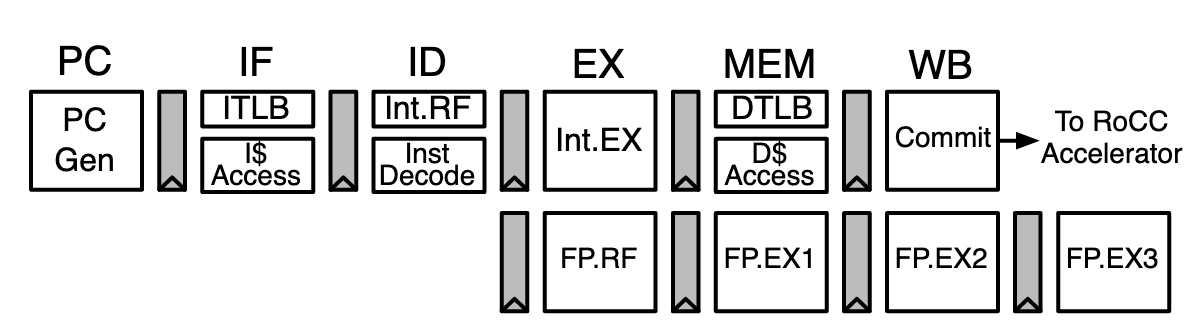
\includegraphics[scale=.4]{pngs/RocketPipeline.png}
%    \caption{Rocket Chkp Pipeline\cite{Asanović:EECS-2016-17}}
%    \label{fig:RocketChipPipeline}
%\end{figure}
The Rocket Core was generated by using the Rocket Chip Generator. The Rocket Chip Generator was developed by UC. Berkeley and is maintained by the CHIPS Alliance. Figure ?? shoe a high level overview of a default Rocket Chip. Starting form top to bottom: The Generator can be used to create N Number of Tiles. Tiles are the most basic 
\subsubsection{LSTM}
\blindtext
\subsubsection{SCNN}
\blindtext
\end{document}

